\documentclass{replab}
\usepackage{lipsum}
\usepackage[shortlabels]{enumitem}

% --- Información del documento ---
\title{Taller - Semana 5}
\author{Diego Alejandro Heredia Franco}

% Nota: Si se desea incluir más de un autor en el documento, el archivo replab.cls, en la sección "Página de título de documento", contiene líneas de código comentadas pensadas para introducir los datos desde 1 hasta 4 autores. Sin embargo, debe escogerse solo una de las cuatro secciones de código y comentar las demás para mantener la consistencia del documento.

\date{30 de abril de 2025}
\subtitle={Física - Geometría}
\email={\href{mailto:dherediaf@unal.edu.co}{\color{principaluno}\texttt{dherediaf@unal.edu.co}}}
\subject={Taller Fundamentos de Mecánica}

\setlength{\columnsep}{14pt}

% --- Archivo de bibliografía ---
\addbibresource{repbib.bib}

% --- Inicio del documento ---
\begin{document}
\setlength{\parindent}{0pt}
	
	\pagestyle{fancy}
	\unspacedoperators
	
% --- Título ---
	{\begin{tcolorbox}[colframe=white, colback=principaldos, arc=8pt]
		\begin{center}
			\maketitle
			%\rule{\textwidth}{0.2pt}
			%\medskip

			%\noindent\textit{Palabras Clave:} medidas directas e indirectas, análisis estadístico, incertidumbre, calibrador Vernier, balanza.
		\end{center}
	\end{tcolorbox}}
	\selectlanguage{spanish}

{\begin{tcolorbox}[colframe=red!50!black, colback=red!5!white, arc=8pt]
	\textbf{Sugerencia:} En el libro \textit{Física para Ciencias e Ingeniería} (Serway) \cite{serway}, se presenta al final de cada capitulo un \textit{\textbf{resumen de los conceptos más importantes}}, así como un pequeño manuscrito con un \textit{\textbf{paso a paso general para resolver problemas}}. Se recomienda al estudiante leer este instructivo para que pueda resolver los ejercicios de forma más organizada y eficiente.
\end{tcolorbox}}

% --- Cuerpo del reporte ---
	\section{\textit{FPS} vs Movimiento Continuo}

	En películas cinematográficas y de televisión es común observar los neumáticos de los vehículos girando en sentido contrario a lo esperado. El efecto se debe a que el registro cinematográfico no es continuo y permanente, sino que se realiza típicamente a razón de $24$ imágenes por segundo ($24$ FPS).

	\begin{enumerate}[a)]
		\item ¿Cúal es la rapidez aparente de un automóvil cuyos neumáticos de $60cm$ de diámetro parecen girar en retroceso a razón de $\pi/3$ radianes por segundo? (R: $-1.13km/h$)
		\item ¿Cúal puede ser la rapidez real del automóvil? Haga un esquema que ilustre la situación? (R: $143\pi/3 rad/s$)
		\item ¿Es posible que el efecto estroboscópico haga que su respuesta no sea unívoca, es decir, que existan otras velocidades que también cumplan con el enunciado del problema? Haga un comentario al respecto.
	\end{enumerate}


	\section{Libra Fuerza y Slug}
	El sistema técnico inglés de medidas define la unidad de fuerza como el peso de una libra masa ($0,453 kg$) y recibe también el nombre de libra. Por su parte, se define la unidad de masa el slug como la masa que acelera a razón de 1 pie/s2 cuando se le aplica una fuerza de una libra. 

	\begin{enumerate}[a)]
		\item ¿Cuánto vale la aceleración de gravedad en el sistema 
		técnico inglés?
		\item ¿A cuántas libras equivale el slug? (R: $32.2$ lb)
	\end{enumerate}

	\section{Trofeo a lo Grande}
	Se desea elaborar una réplica ampliada tres veces de un trofeo que descansa en un pedestal que apenas sí soporta al trofeo. ¿En qué factor se afectan las dimensiones lineales del nuevo pedestal respecto del original, para apenas soportar la réplica?
	\textit{\textbf{Nota:}} El trofeo ampliado se fabricará con el mismo material que el original. \\
	
	\textit{\textbf{Sugerencia:}} Puede intentar primero resolver el problema para un trofeo de forma regular (e.g. un cilindro o un paralelepípedo) y luego generalizarlo para cualquier forma.

	\section{Ley Cuadrático - Cúbica}
	Tome dos figuras de su elección (e.g. cono, cilindro, etc.) y estudie como varia su área y volumen conforme se amplia su tamaño en un factor lineal de $n$. Haga gráficos de las áreas y volúmenes, así como de la razón $V/A$ en función de la escala $n$ ¿Qué observa? Averigüe sobre la ley cuadrático-cúbica (ver figura \ref{fig:galileo}) y sus implicaciones en ingeniería y biología ¿Por qué es importante para el diseño de estructuras?

	\begin{figure}[htbp]
		\centering
		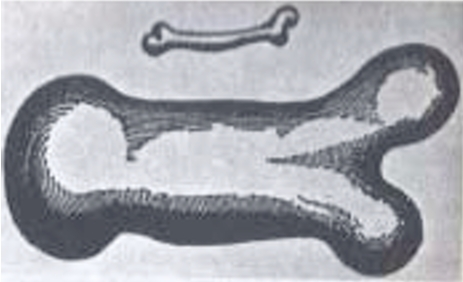
\includegraphics[width=.5\columnwidth]{imagenes/galileo.jpeg}
		\caption{Dibujo esquemático de la ley cuadrático-cúbica.}
		\label{fig:galileo}
	\end{figure}


	\section{Analogía: Ley de la Inversa del Cuadrado}

	\begin{figure}[htbp]
		\centering
		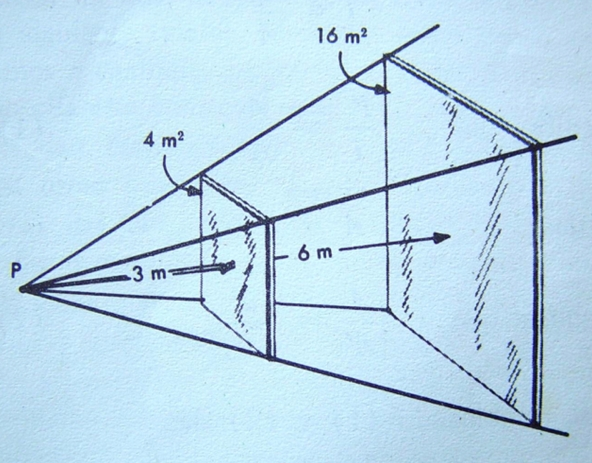
\includegraphics[width=.5\columnwidth]{imagenes/r-2.jpeg}
		\caption{Dibujo esquemático de la ley de la inversa del cuadrado.}
		\label{fig:r-2}
	\end{figure}

	En clase se analizó el origen de la dependencia del tipo cuadrado inverso con la distancia, como una consecuencia de la conservación del flujo de energía o de partículas que, emanadas o emitidas por una fuente $P$, se propagan en línea recta a través del espacio (figura \ref{fig:r-2}). Por analogía, discuta la dependencia con la distancia del flujo de agua que vierte un surtidor sobre la rampa circular en forma de paraguas que ilustra la figura \ref{fig:r-1} (un cono de apertura angular $\theta$) suponiendo que el líquido desciende suave y homogéneamente, con simetría circular desde la boquilla del surtidor. \textit{\textbf{Nota:}} La boquilla es tan pequeña que puede considerarse de tamaño puntual. 

	\begin{enumerate}[a)]
		\item ¿Cuál es la dependencia con r de la cantidad de agua en mililitros por segundo y por centímetro de arco $f(mL/(s\cdot cm)$, que fluye cuesta abajo, conociendo la cantidad de agua $f_0(ml/s)$ que vierte la boquilla.
		\item ¿Cuál es la constante de proporcionalidad asociada a 
		dicha dependencia?
	\end{enumerate}

	\begin{figure}[htbp]
		\centering
		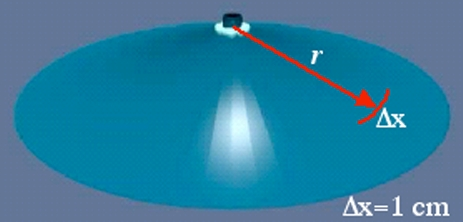
\includegraphics[width=.5\columnwidth]{imagenes/r-1.jpeg}
		\caption{Dibujo esquemático de la rampa circular.}
		\label{fig:r-1}
	\end{figure}

	\printbibliography[heading=bibintoc]
	
\end{document}